%%%%%%%%%%%%%%%%%%%%%%%%%%%%%%%%%%%%%%%%%%%%%%%%%%%%%%%%%%%%%%%%%%%%%%%
%%%%%%%%%%%%%%%%%%%%%%%%%%%%%%%%%%%%%%%%%%%%%%%%%%%%%%%%%%%%%%%%%%%%%%%
%%%%%                                                                 %
%%%%%     <file_name>.tex                                             %
%%%%%                                                                 %
%%%%% Author:      <author>                                           %
%%%%% Created:     <date>                                             %
%%%%% Description: <description>                                      %
%%%%%                                                                 %
%%%%%%%%%%%%%%%%%%%%%%%%%%%%%%%%%%%%%%%%%%%%%%%%%%%%%%%%%%%%%%%%%%%%%%%
%%%%%%%%%%%%%%%%%%%%%%%%%%%%%%%%%%%%%%%%%%%%%%%%%%%%%%%%%%%%%%%%%%%%%%%

\chapter{Task Description}
Include the task description \textbf{pdf} you got from your
assistant(s) with the \shell{\textbackslash includepdf} command.
% include the task description pdf!

\includepdf[pages={2-}, pagecommand={\thispagestyle{headings}}, turn=false, scale=0.9]{../task.pdf}

\chapter{Declaration of Authorship}
Include the declaration of authorship (\url{http://www.ethz.ch/faculty/exams/plagiarism/}) with the \shell{\textbackslash includepdf} command
(sign it and scan it).
% include the signed declaration of authorship!
%\includepdf[pages=-, turn=false, scale=0.9]{... .pdf}


\chapter{File Structure}
Describe how the project directories/files are organized, e.g.:

\begin{flushleft}
\dirtree{%
.1 /.
  .2 README \DTcomment{A README with some general information about the project.}.
  .2 01\_report \DTcomment{The source files of the project report.}.
  .2 02\_presentation \DTcomment{The source files of the presentation.}.
  .2 03\_designflow \DTcomment{Some designflow-specific files.}.
.2 03\_designflow \DTcomment{Some designflow-specific files.}.
  .3 03\_designflow \DTcomment{Some designflow-specific files.}.
}
\end{flushleft}

What needs to be done to run an RTL simulation (stimuli generation,
compilation...)?


\chapter{Datasets}
If you have a data set comprising several test images, you could
depict and describe them here. Use a simple naming scheme such that
you can easily refer to certain elements of this data set in the text.


\chapter{More Evaluation Results}
If you conducted an extensive evaluation you could move surplus
graphs/results to the appendix.


\chapter{Algorithms / Tables}
Large algorithm boxes and tables may clutter your chapters and impair
the readability. If they are not very important, consider moving them
to the appendix as well.


\chapter{ASIC Datasheet ($<$OR10N$>$)}

TODO: Some description about OR10N

\minitoc

\section{Features}
\begin{itemize}
\item OpenRISC 1200 32-Bit architecture.
\item 72 \gls{orbis} instructions. (see Table \ref{tab:instr})
\item Additional instruction for End of Computation. (l.cust1)
\item 33-bit signed (hardware) multiplier.
\item Debugging interface. Messages can be printed character-wise on Data Output.
\item Test interface for cache misses.
\item Full Scan-Chain (Flaw detection)
\end{itemize}

\section{Applications}
\lipsum[2]

\section{Description}
\lipsum[2]

\section{Packaging}
Package QFN56 is used with 16 power pins and 40 user pins.

\section{Bonding Diagram}
The 16 power pins and the clock pin are arranged the same way as it is on the  Standard QFN56 tester board. See Figure \ref{fig:bonding} for more details.
\begin{figure}[htbp]

  \centering 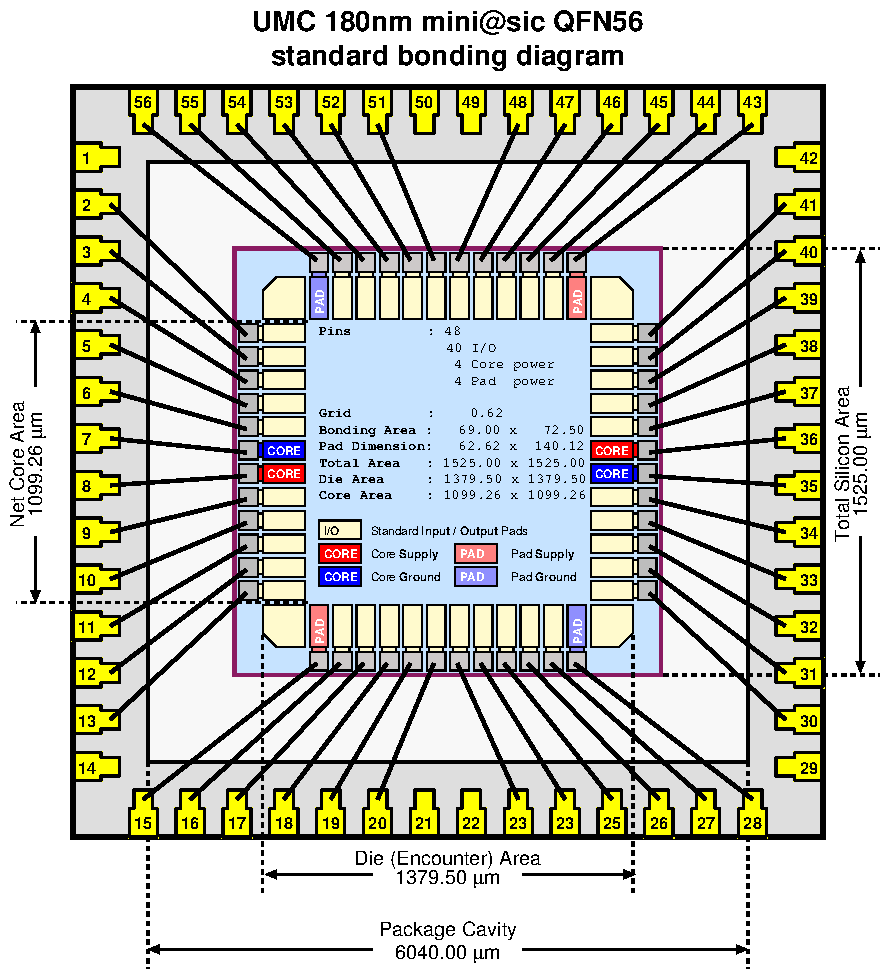
\includegraphics[width=0.9\textwidth]{./figures/qfn56_180_std}
  \caption{Bonding diagram.}
\label{fig:bonding}
\end{figure}
\clearpage
\section{Pin Map}

\begin{figure}[!htbp]
  \centering 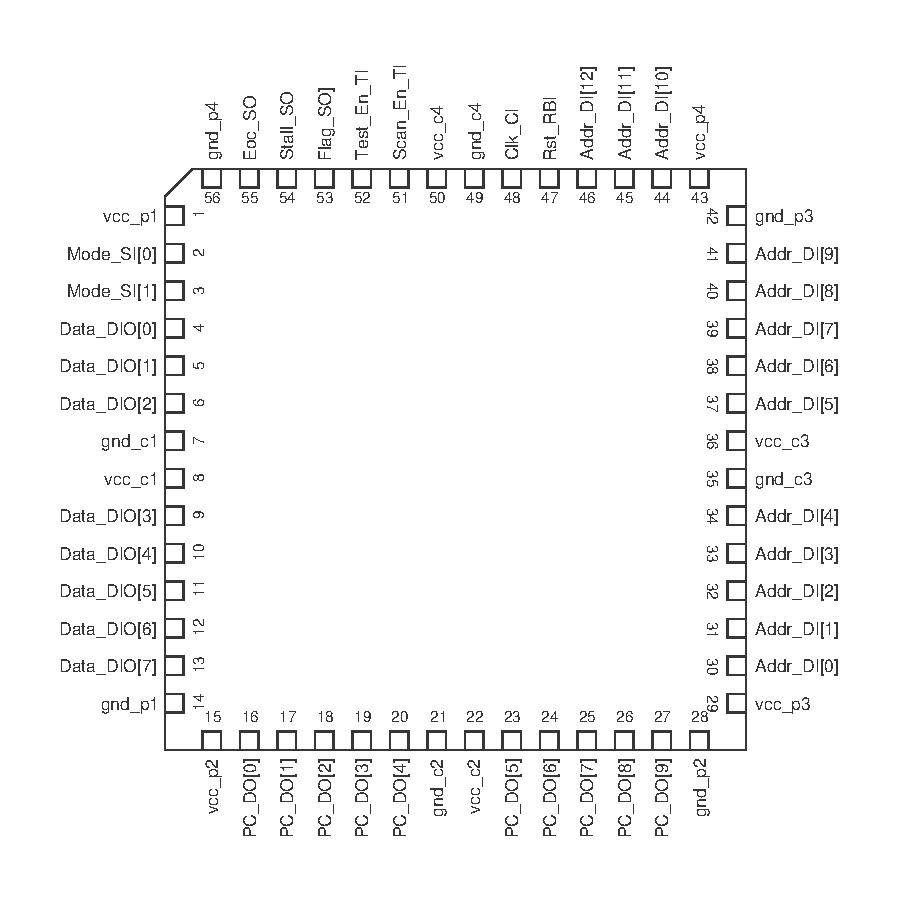
\includegraphics[width=1.0\textwidth]{./figures/asic_pinout}
  \caption{$<$OR10N$>$ pinout.}
\end{figure}

\section{Pin Description}
Table \ref{tab:power_pins} and table \ref{tab:pins} describe the usage of the power pins and user pins respectively.
\begin{table}[!tbph]
 \caption{Power Pins}
 \label{tab:power_pins}
 \centering\begin{tabular}{|r| l| l|} \hline
14; 28; 42; 56 & gnd\_p & Pad Ground \\ \hline
01; 15; 29; 43 & vcc\_p & Pad Supply \\ \hline
07; 21; 35; 49 & gnd\_c & Core Ground \\ \hline
08; 22; 36; 50 & vcc\_c & Core Supply \\ \hline
 \end{tabular}

\end{table}
\begin{landscape}
\begin{savenotes}
\begin{table}[htbp]
 \caption{User-Defined pins. (IO, Clock, Reset, Test)}
 \label{tab:pins}
 \centering\begin{tabular}{|r| p{3cm}|p{3cm} |p{3cm} |p{3cm}|p{3cm}|} \hline
No. & Name & Setup &Run & Readout & Test \\ \hline
2-3 & Mode\_SI & \multicolumn{4}{ |l| }{Defines Mode. See \ref{sec:mode} for further information.} \\ \hline
4-6; 9-13 & Data\_DIO & Data Input to\newline memories & Debugging\newline Output (qprint) & Data Output\newline from memories & - \\ \hline
16-20; 23-27 & PC\_DO & - & \gls{pc} in \gls{id} stage & - & Scan\_In\_TI \\ \hline
30-34;37-41 & Addr\_DI[9:0] & \multirow{4}{*}{Memory Address}  & - &\multirow{4}{*}{Memory Address} & Scan\_Out\_TO \\ 
44 & Addr\_DI[10] & & - & & - \\
45 & Addr\_DI[11] & & Instr\_Ack\_TI\footnote{If set to 0 a cache miss from the instruction memory will occur.} &  & - \\ 
46 & Addr\_DI[12] &  & Data\_Ack\_TI\footnote{If set to 0 a cache miss from the data memory will occur.}  &  & - \\ \hline
47 & Rst\_RBI & \multicolumn{4}{|l|}{Reset signal. (Active low)} \\ \hline
48 & Clk\_CI & \multicolumn{4}{|l|}{Clock Signal} \\ \hline
51 & Scan\_En\_TI &- &- &- & Scan Enable \\ \hline
52 & Test\_En\_TI &- &- &- & Test Enable \\ \hline
53 & Flag\_SO &- & Flag Signal &- &- \\ \hline
54 & Stall\_SO &- & Stall Signal &- &- \\ \hline
55 & Eoc\_SO &- & End of Computation signal &- &- \\ \hline
 \end{tabular}
\end{table}
\end{savenotes}
\end{landscape}
 
\section{Interface Description}


\section{Register Map}

\section{Memory Addressing}
\label{sec:mem_addr}
Data can be written or read bytewise from chip. Internally data are stored wordwise (4 Bytes). The memory addressing scheme is illustrated in Table \ref{tab:addr_scheme} and table \ref{tab:byteorder} shows the Byte Addressing. 
\begin{table}[htbp]
 \caption{Address scheme}
 \label{tab:addr_scheme}
\centering\begin{tabular}{|l| l|} \hline
 \multirow{2}{*}{Addr\_DI[12]} & 0 points to the instruction memory \\ 
                               & 1 points to the data memory \\ \hline
 Addr\_DI[11:2] & word address \\ \hline
 Addr\_DI[1:0] & byte address \\ \hline

 \end{tabular}
\end{table}

\begin{table}[htbp]
 \caption{Bit and Byte Ordering. \cite{or1000}}
 \label{tab:byteorder}
\centering\begin{tabular}{|c c|c c|c c|c c|} \hline
 Bit 31 & Bit 24 & Bit 23 & Bit 16 & Bit 15 & Bit 8 & Bit 7 & Bit 0 \\ \hline
\multicolumn{2}{|c|}{MSB} & & & & & \multicolumn{2}{|c|}{LSB} \\ \hline
\multicolumn{2}{|c|}{Byte Address 00} & \multicolumn{2}{|c|}{Byte Address 01} & \multicolumn{2}{|c|}{Byte Address 10} & \multicolumn{2}{|c|}{Byte Address 11} \\ \hline 

 \end{tabular}
\end{table}



\section{Operation Modes}
\label{sec:mode}
OR10N runs in 4 different operational modes and 1 test mode. Table \ref{tab:pins} shows pin usage for all functional modes separately.
\subsection{Functional Modes}
\subsubsection{IDLE}
CPU is in IDLE mode if Mode\_SI[1:0] is set to 00.\\
CPU is disabled, memories are not written. The chip drives the bidirectional signal Data\_DIO to all zero.
\subsubsection{SETUP}  
CPU is in SETUP state if Mode\_SI[1:0] is set to 10.\\
In this mode the data can be written from outside to both of the memories. Data is laid bytewise to the bidirectional pin Data\_DIO and is saved at address Addr\_DI on rising edge.  Section \ref{sec:mem_addr} explains how the bytes are addressed.
\subsubsection{RUN}
CPU is in RUN mode if Mode\_SI[1:0] is set to 01.\\
Main Mode. CPU runs until end of computation is reached (special signal l.cust1), then signal Eoc\_SO is set to 1. During RUN state some outputs can be used for debugging.
\begin{itemize}
\item PC\_DO: Current \gls{pc} in \gls{id} stage.
\item Data\_DIO: Is either 0 or an ASCII character. Can be printed out using qprint (C programs) or writing to address 0x1FFF (Assembler).
\item Flag\_SO: Current Flag.
\item Stall\_SO: Indicates whether there is a stall at this time. 
\item Eoc\_SO: Indicates that the end of the program were reached.
\end{itemize}

Although no misses can occur on this chip, there is a possibility to inject a delibarate miss to check cpu's ability for handling them. The following inputs are used for this option.
\begin {itemize}
\item Addr\_DI[11]=Instr\_Ack\_TI: If this signal is set to 0, the instruction memory will cause a miss in the next cycle.
\item Addr\_DI[12]=Data\_Ack\_TI: If this signal is set to 0, the data memory will cause a miss in the next cycle.
\end{itemize}

\subsubsection{READOUT}
CPU is in RUN mode if Mode\_SI[1:0] is set to 11.\\
In the READOUT mode both memories can be read out using the address scheme from section \ref{sec:mem_addr}. The byte at address Addr\_DI is read from memory and put on Data\_DIO with one latency. 

\subsection{Test Modes}
If Test\_En\_TI is set to 1 both memory macrocells are bypassed. This allows a better test coverage using ATPG. See schema TODO for more information.


\section{Electrical Specifications}
\begin{table}[htbp]
 \caption{DC characteristics \cite{faraday}}
 \label{tab:elect_rec}
\centering\begin{tabular}{|l|l|r|r|c|} \hline
Symbol & Description & Min. & Max. & Unit \\ \hline
$V_{Il}$ & Input low voltage & - & 0.8 & $V$ \\ \hline
$V_{Ih}$ & Input high voltage & 2.0 & - & $V$ \\ \hline
$V_{Ol}$ & Output low voltage & - & 0.4 & $V$ \\ \hline
$V_{Oh}$ & Output high voltage & 2.4 & - & $V$ \\ \hline
$I_O$ & Output driving & \multicolumn{2}{r|}{8} & $mA$ \\ \hline

 \end{tabular}
\end{table}

\subsection{Recommended Operating Regions}
\begin{table}[htbp]
 \caption{Recommended Operating Conditions \cite{faraday}}
 \label{tab:elect_rec}
\centering\begin{tabular}{|l|l|r|r|r|c|} \hline
Symbol & Description & Min. & Typ. & Max. & Unit \\ \hline
\textit{vcc\_c} & Core power supply & 1.62 & 1.8 & 1.98 & $V$ \\ \hline
\textit{vcc\_p} & Pad power supply & 2.97 & 3.3 & 3.63 & $V$ \\ \hline
$T_J$ & Operating junction temperature & -40 & 25 & 125 & $^{\circ} C$ \\ \hline

 \end{tabular}
\end{table}

\subsection{Absolute Maximum Ratings}
\begin{table}[htbp]
 \caption{Absolute Maximum Ratings \cite{faraday}}
 \label{tab:elect_rec}
\centering\begin{tabular}{|l|l|c|c|} \hline
Symbol & Description & Rating & Unit \\ \hline
\textit{vcc\_c} & Core power supply & -0.5 $\sim$ 2.5 & $V$ \\ \hline
\textit{vcc\_p} & Pad power suplly & -0.5 $\sim$ 4.6 & $V$ \\ \hline
$V_{In}$ & Input voltage &  -0.5 $\sim$ 4.6 & $^{\circ} C$ \\ \hline
$I_{In}$ & DC input current & 50 & $mA$ \\ \hline
$I_{Out}$ & DC output current & 50 & $mA$ \\ \hline
 \end{tabular}
\end{table}
